\documentclass[11pt,a4paper]{report}
\usepackage[utf8]{inputenc}
\usepackage[left=2cm,right=2cm,top=2cm,bottom=2cm]{geometry}
\usepackage{color}
\definecolor{mygreen}{rgb}{0,0.6,0}
\definecolor{mygray}{rgb}{0.5,0.5,0.5}
\definecolor{mymauve}{rgb}{0.58,0,0.82}
\usepackage[english]{babel}
\usepackage{amsmath}
\usepackage{amsfonts}
\usepackage{amssymb}
\usepackage{mathtools}
\usepackage{tocloft}
\usepackage{listings}
\usepackage{graphicx}
\usepackage{tikz}
\usepackage{bigints}
\usepackage{fourier}
\usepackage{fancyhdr}
\pagestyle{fancy}
\usepackage{dsfont}
\usepackage{units}
\usepackage{textcomp}
\usepackage{subcaption}
\usepackage{parskip}
\usepackage{float}
\usepackage{pdfpages}
\renewcommand{\lstlistlistingname}{Code Listings}
\renewcommand{\lstlistingname}{Code Listing}
\definecolor{gray}{gray}{0.5}
\definecolor{green}{rgb}{0,0.5,0}
\lstset{
	tabsize=4,
	rulecolor=,
	language=python,
	%basicstyle=\ttfamily\scriptsize,
	basicstyle=\footnotesize,
	upquote=true,
	numbers=left,
	numberstyle=\footnotesize,
	aboveskip={1.5\baselineskip},
	extendedchars=true,
	linewidth=\linewidth,
	breaklines=false,
	prebreak=\raisebox{0ex}[0ex][0ex]{\ensuremath{\hookleftarrow}},
	frame=single,
	columns=fullflexible,
	showtabs=false,
	showspaces=false,
	showstringspaces=false,
	identifierstyle=\ttfamily,
	keywordstyle=\color[rgb]{0,0,1},
	commentstyle=\color[rgb]{0.133,0.545,0.133},
	stringstyle=\color[rgb]{0.627,0.126,0.941},
}
\pagestyle{fancy}
\lhead{Travis Mitchell}
\rhead{}
\chead{MECH3750 - Content Summary}
\renewcommand{\headrulewidth}{0.8pt}
\renewcommand{\footrulewidth}{0.8pt}

\author{\textit{Travis Mitchell}}
\title{Lecture Content Summaries for MECH3750}
\date{Updated: 13 September, 2019}			

\makeatletter
\newcommand*{\toccontents}{\@starttoc{toc}}
\makeatother
\renewcommand{\thesection}{\thepart \arabic{section}}


\begin{document}
	\maketitle
	\clearpage
	
	%% WEEK 02
	\begingroup
	\makeatletter
	\let\clearpage\relax
	\vspace*{\fill}
	\vspace*{\dimexpr-50\p@-\baselineskip}
	\chapter*{Week 02}
	With thanks to Alex Muirhead: \\\\
	\textbf{Tutors:} Alex Muirhead, Bryce Hill, Kyle Mclaren, Luke Bartholomew, William Snell \\\\
	\textbf{Quizzes:} Weeks 3, 6, 9 \\\\	
	\textbf{Content:}
	\begin{itemize}
		\item Taylor Expansions;
		\item Newton's Method;
		\item Least Squares.
	\end{itemize}
	\vspace*{\fill}
	\endgroup
	\includepdf[pages={2-}]{wk02/Week02-TaylorExpansions-NewtonsMethod-LeastSquares.pdf}
	
	
	%% WEEK 03
	\begingroup
	\makeatletter
	\let\clearpage\relax
	\vspace*{\fill}%
	\vspace*{\dimexpr-50\p@-\baselineskip}
	\chapter*{Week 03}
	With thanks to Alex Muirhead: \\\\
	\textbf{Tutors:} Alex Muirhead, Bryce Hill, Kyle Mclaren, Luke Bartholomew, William Snell \\\\
	\textbf{Quiz:} Weeks 3 - 1pm \\\\	
	\textbf{Content:}
	\begin{itemize}
		\item Least Squares continued;
		\item Inner product;
		\item Orthogonal polynomials;
		\item Fourier Series.
	\end{itemize}
	\vspace*{\fill}
	\endgroup
	\includepdf[pages={2-}]{wk03/Week03-LeastSquaresCont-InnerProduct-OrthogonalPolynomials-FourierSeries.pdf}
	
	%% WEEK 04
	\begingroup
	\makeatletter
	\let\clearpage\relax
	\vspace*{\fill}%
	\vspace*{\dimexpr-50\p@-\baselineskip}
	\chapter*{Week 04}
	\textbf{Tutors:} Luke Bartholomew, Bryce Hill, Kyle Mclaren, Travis Mitchell, Alex Muirhead, William Snell \\\\
	\textbf{Assessment:} 
	\begin{itemize}
		\item Quiz 1 results are available for collection;
		\item Next quiz week 6;
		\item Assignment 1 due week 7.
	\end{itemize}	
	\textbf{Content:}
	\begin{itemize}
		\item Fourier series continued;
		\item Discrete Fourier Series.
	\end{itemize}
	\vspace*{\fill}
	\endgroup
	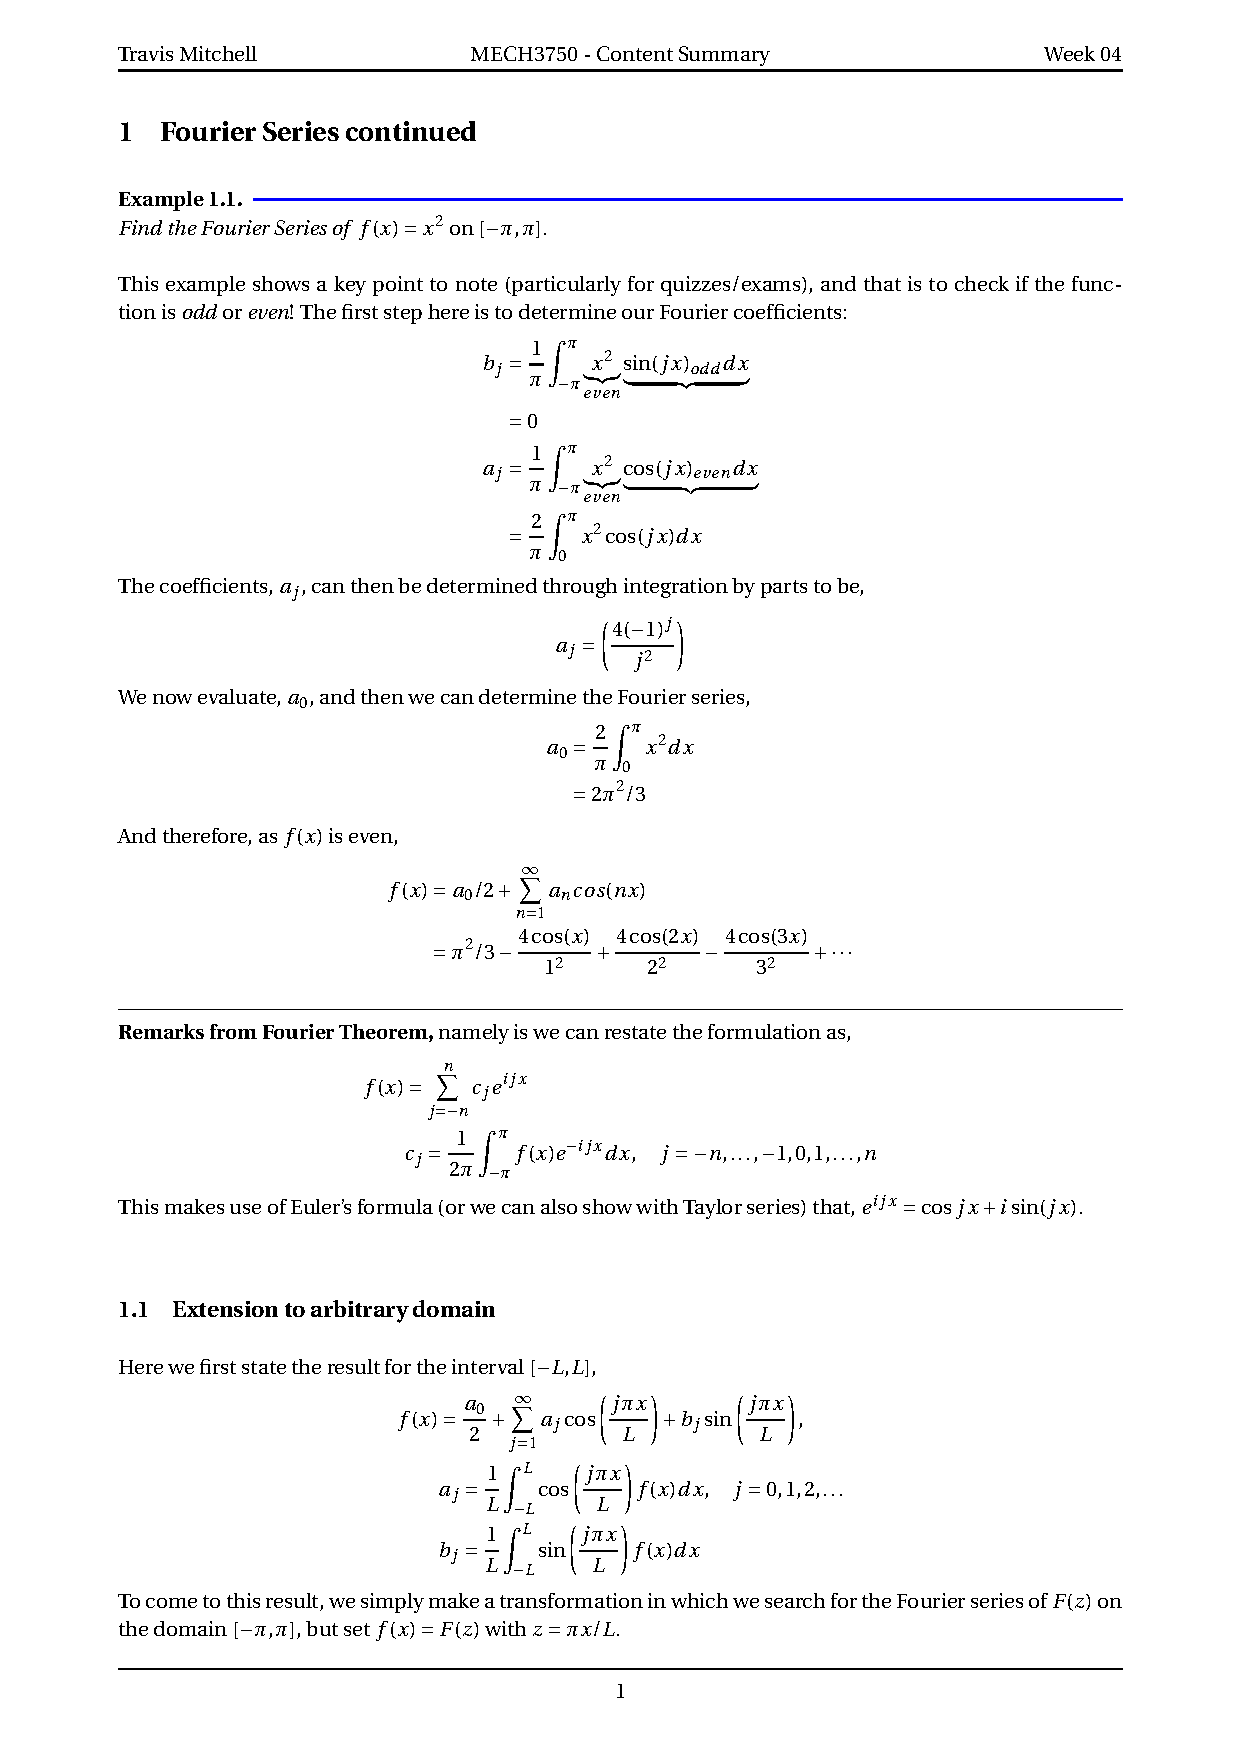
\includepdf[pages={1-}]{wk04/Week04.pdf}
	
		%% WEEK 04
	\begingroup
	\makeatletter
	\let\clearpage\relax
	\vspace*{\fill}%
	\vspace*{\dimexpr-50\p@-\baselineskip}
	\chapter*{Week 05}
	\textbf{Tutors:} Luke Bartholomew, Nathan di Vaira, Bryce Hill, Kyle Mclaren, Travis Mitchell, Alex Muirhead, William Snell \\\\
	\textbf{Assessment:} 
	\begin{itemize}
		\item Next quiz week 6;
		\item Assignment 1 due week 7.
	\end{itemize}	
	\textbf{Content:}
	\begin{itemize}
		\item Introduction to PDEs;
		\item Introduction to separation of variables.
	\end{itemize}
	\vspace*{\fill}
	\endgroup
	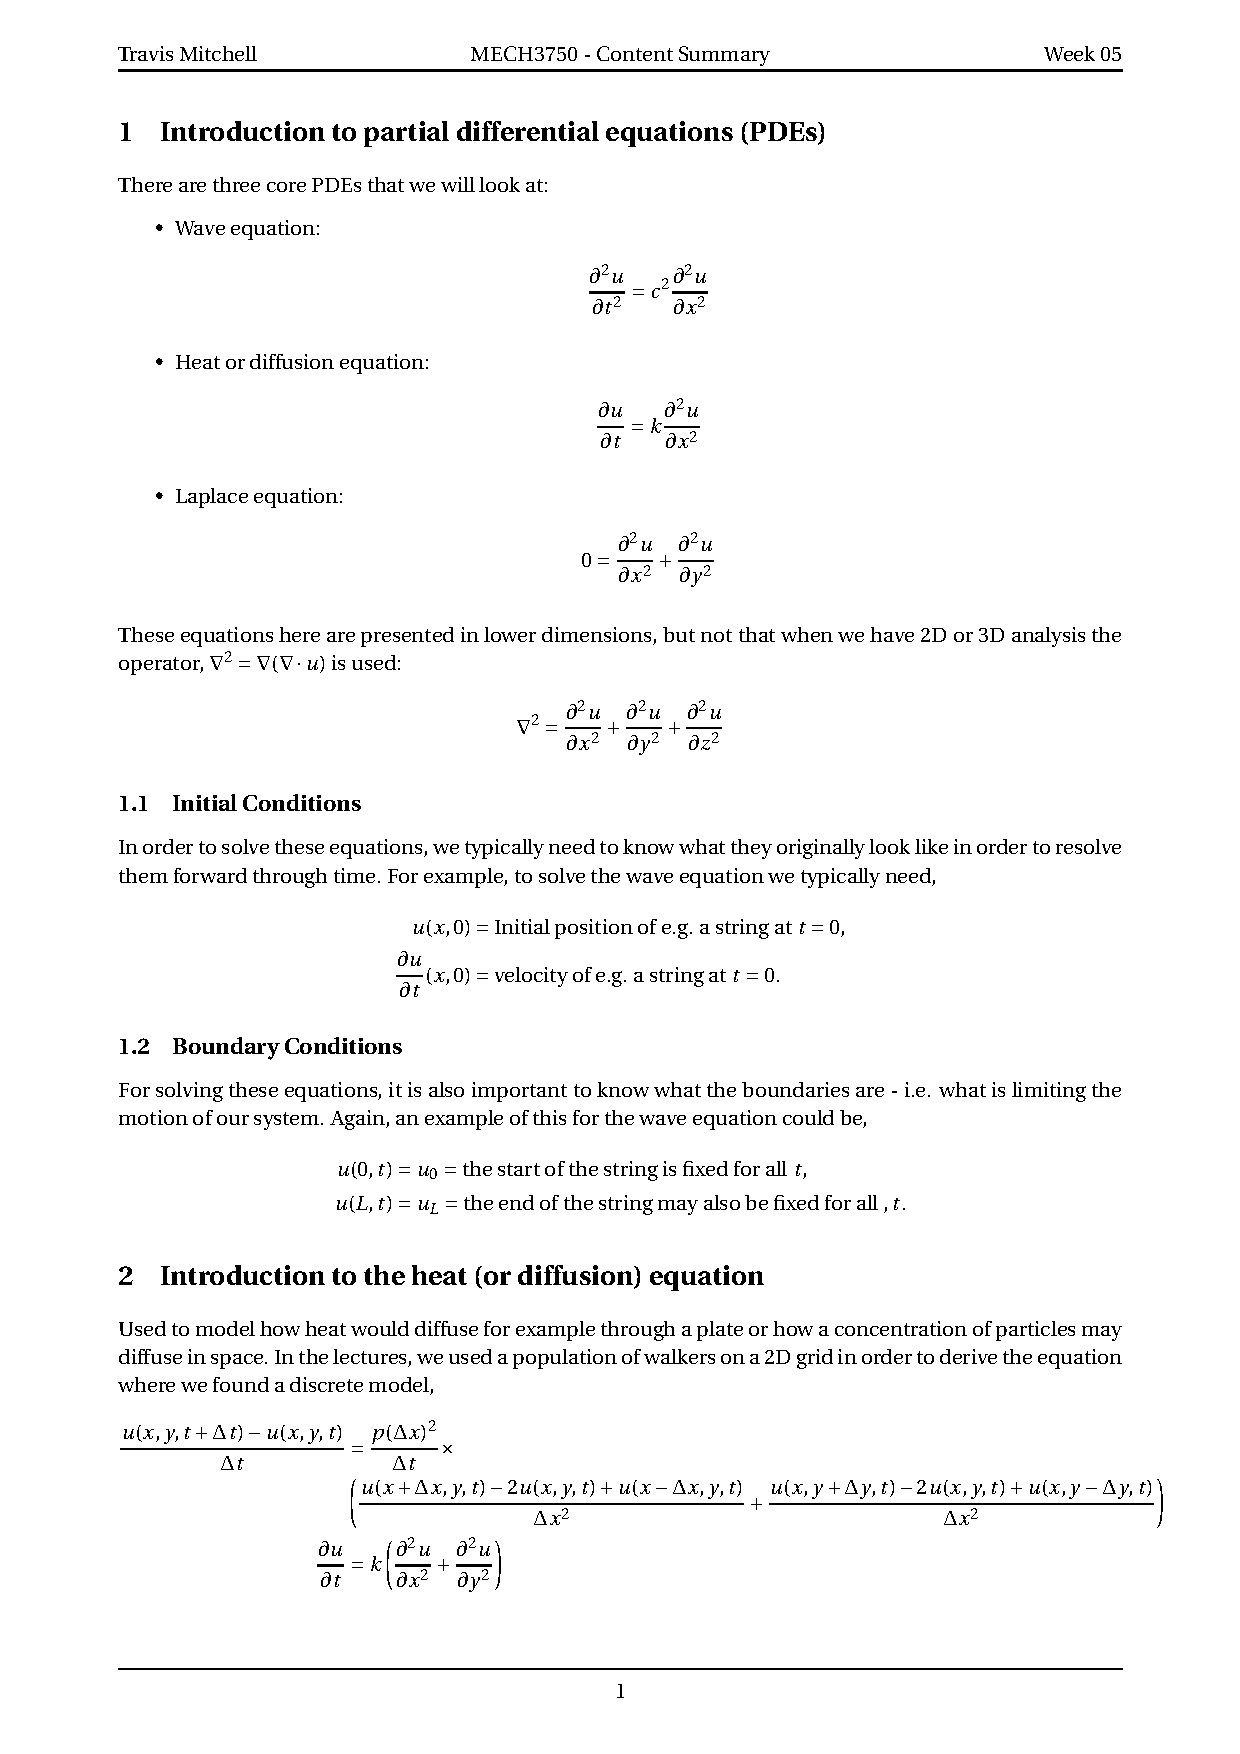
\includepdf[pages={1-}]{wk05/Week05.pdf}
	
		\begingroup
	\makeatletter
	\let\clearpage\relax
	\vspace*{\fill}%
	\vspace*{\dimexpr-50\p@-\baselineskip}
	\chapter*{Week 06}
	\textbf{Tutors:} Luke Bartholomew, Nathan di Vaira, Bryce Hill, Kyle Mclaren, Travis Mitchell, Alex Muirhead, William Snell \\\\
	\textbf{Assessment:} 
	\begin{itemize}
		\item Next quiz TODAY!;
		\item Assignment 1 due week 7.
	\end{itemize}	
	\textbf{Content:}
	\begin{itemize}
		\item Separation of variables.
	\end{itemize}
	\vspace*{\fill}
	\endgroup
	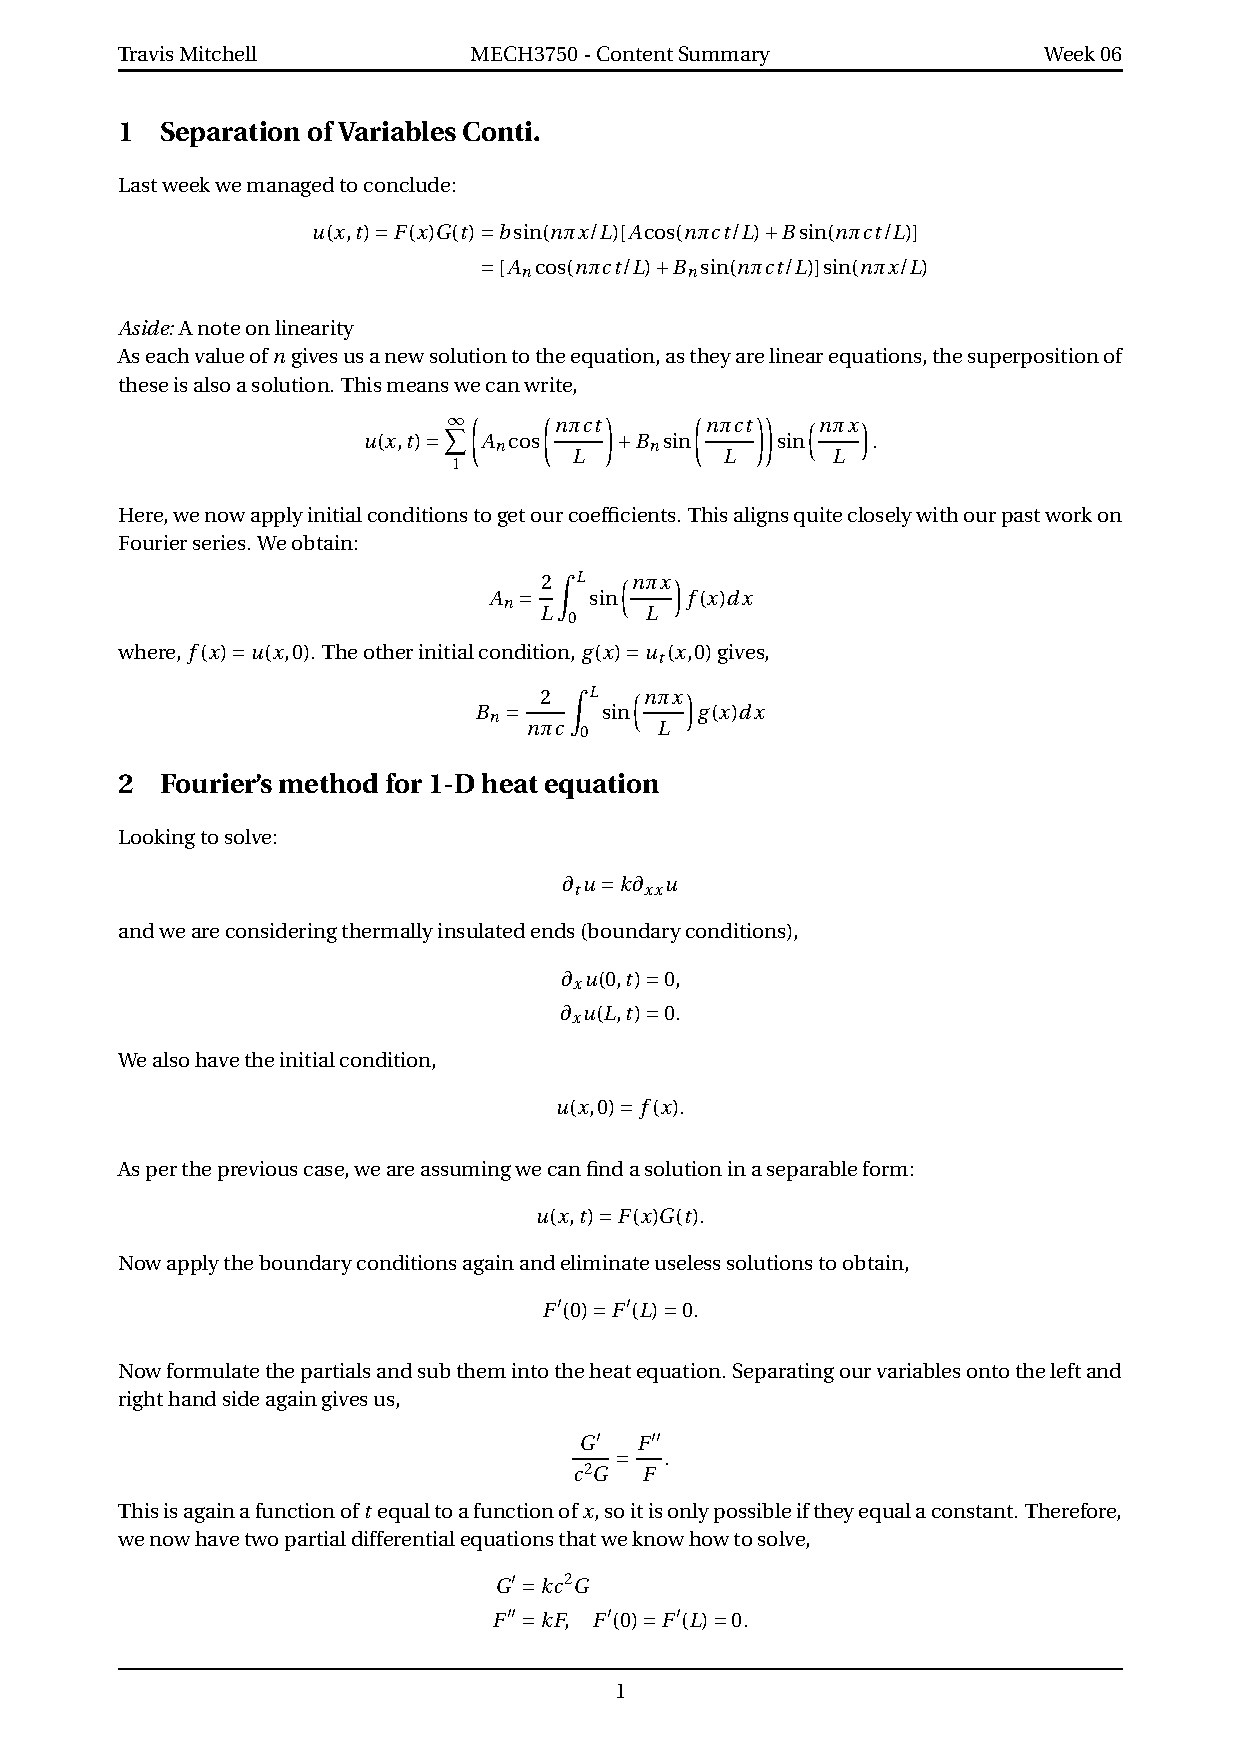
\includepdf[pages={1-}]{wk06/Week06.pdf}
	
	
	\begingroup
	\makeatletter
	\let\clearpage\relax
	\vspace*{\fill}%
	\vspace*{\dimexpr-50\p@-\baselineskip}
	\chapter*{Week 07}
	\textbf{Tutors:} Luke Bartholomew, Nathan di Vaira, Bryce Hill, Kyle Mclaren, Travis Mitchell, Alex Muirhead, William Snell \\\\
	\textbf{Assessment:} 
	\begin{itemize}
		\item Collect your quiz results;
		\item Hopefully you have submitted your assignment;
		\item Next quiz is in Week 9;
		\item Next assignment isn't until Week 12. 
	\end{itemize}	
	\textbf{Content:}
	\begin{itemize}
		\item Started Part II of the course! Well done making it through Part I;
		\item Classification of PDEs;
		\item Numerical solutions to PDEs.
	\end{itemize}
	\vspace*{\fill}
	\endgroup
	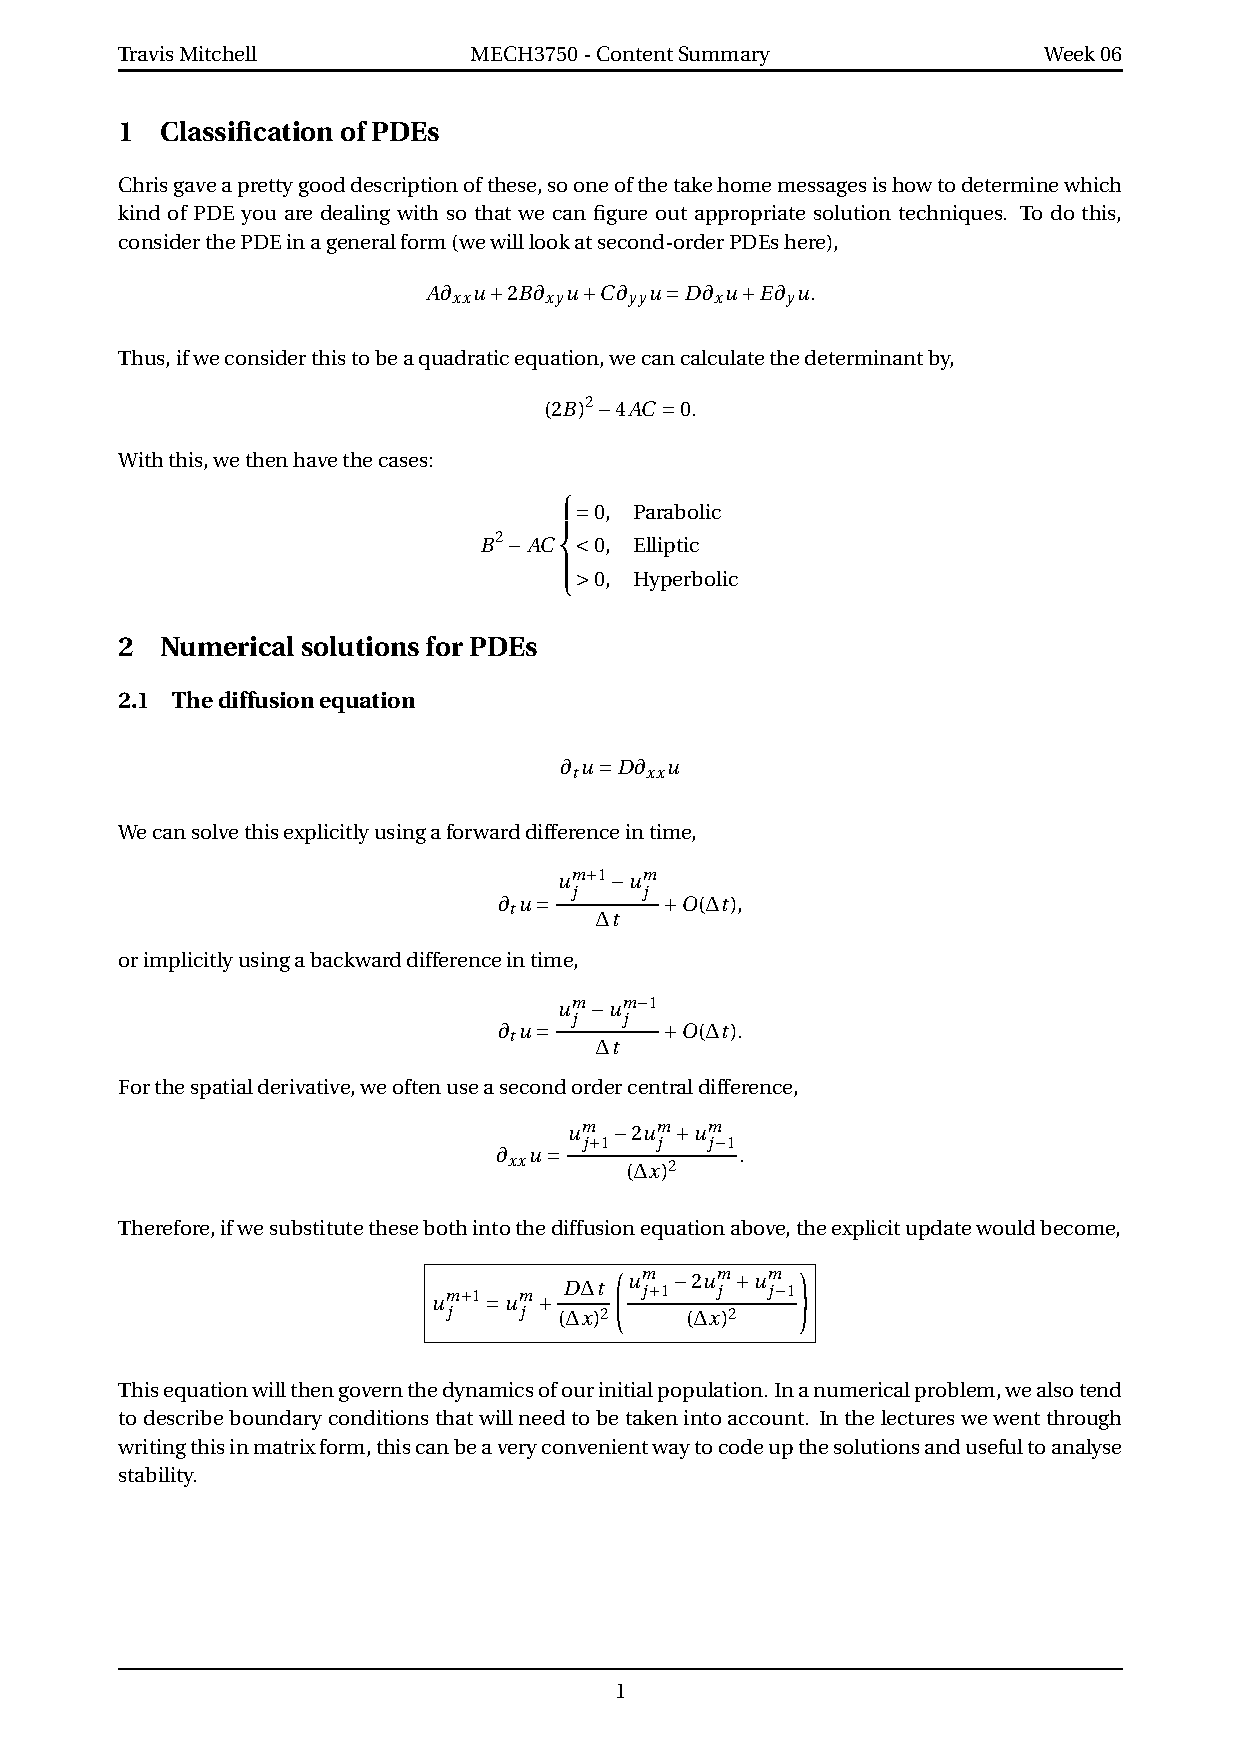
\includepdf[pages={1-}]{wk07/Week07.pdf}
	
	
	\begingroup
	\makeatletter
	\let\clearpage\relax
	\vspace*{\fill}%
	\vspace*{\dimexpr-50\p@-\baselineskip}
	\chapter*{Week 08}
	\textbf{Tutors:} Luke Bartholomew, Nathan di Vaira, Bryce Hill, Kyle Mclaren, Travis Mitchell, Alex Muirhead, William Snell \\\\
	\textbf{Assessment:} 
	\begin{itemize}
		\item Next quiz is in Week 9;
		\item Next assignment due in Week 12. 
	\end{itemize}	
	\textbf{Content:}
	\begin{itemize}
		\item Backwards difference schemes and stability;
		\item Boundary conditions and implementation;
		\item Crank-Nicolson scheme.
	\end{itemize}
	\vspace*{\fill}
	\endgroup
	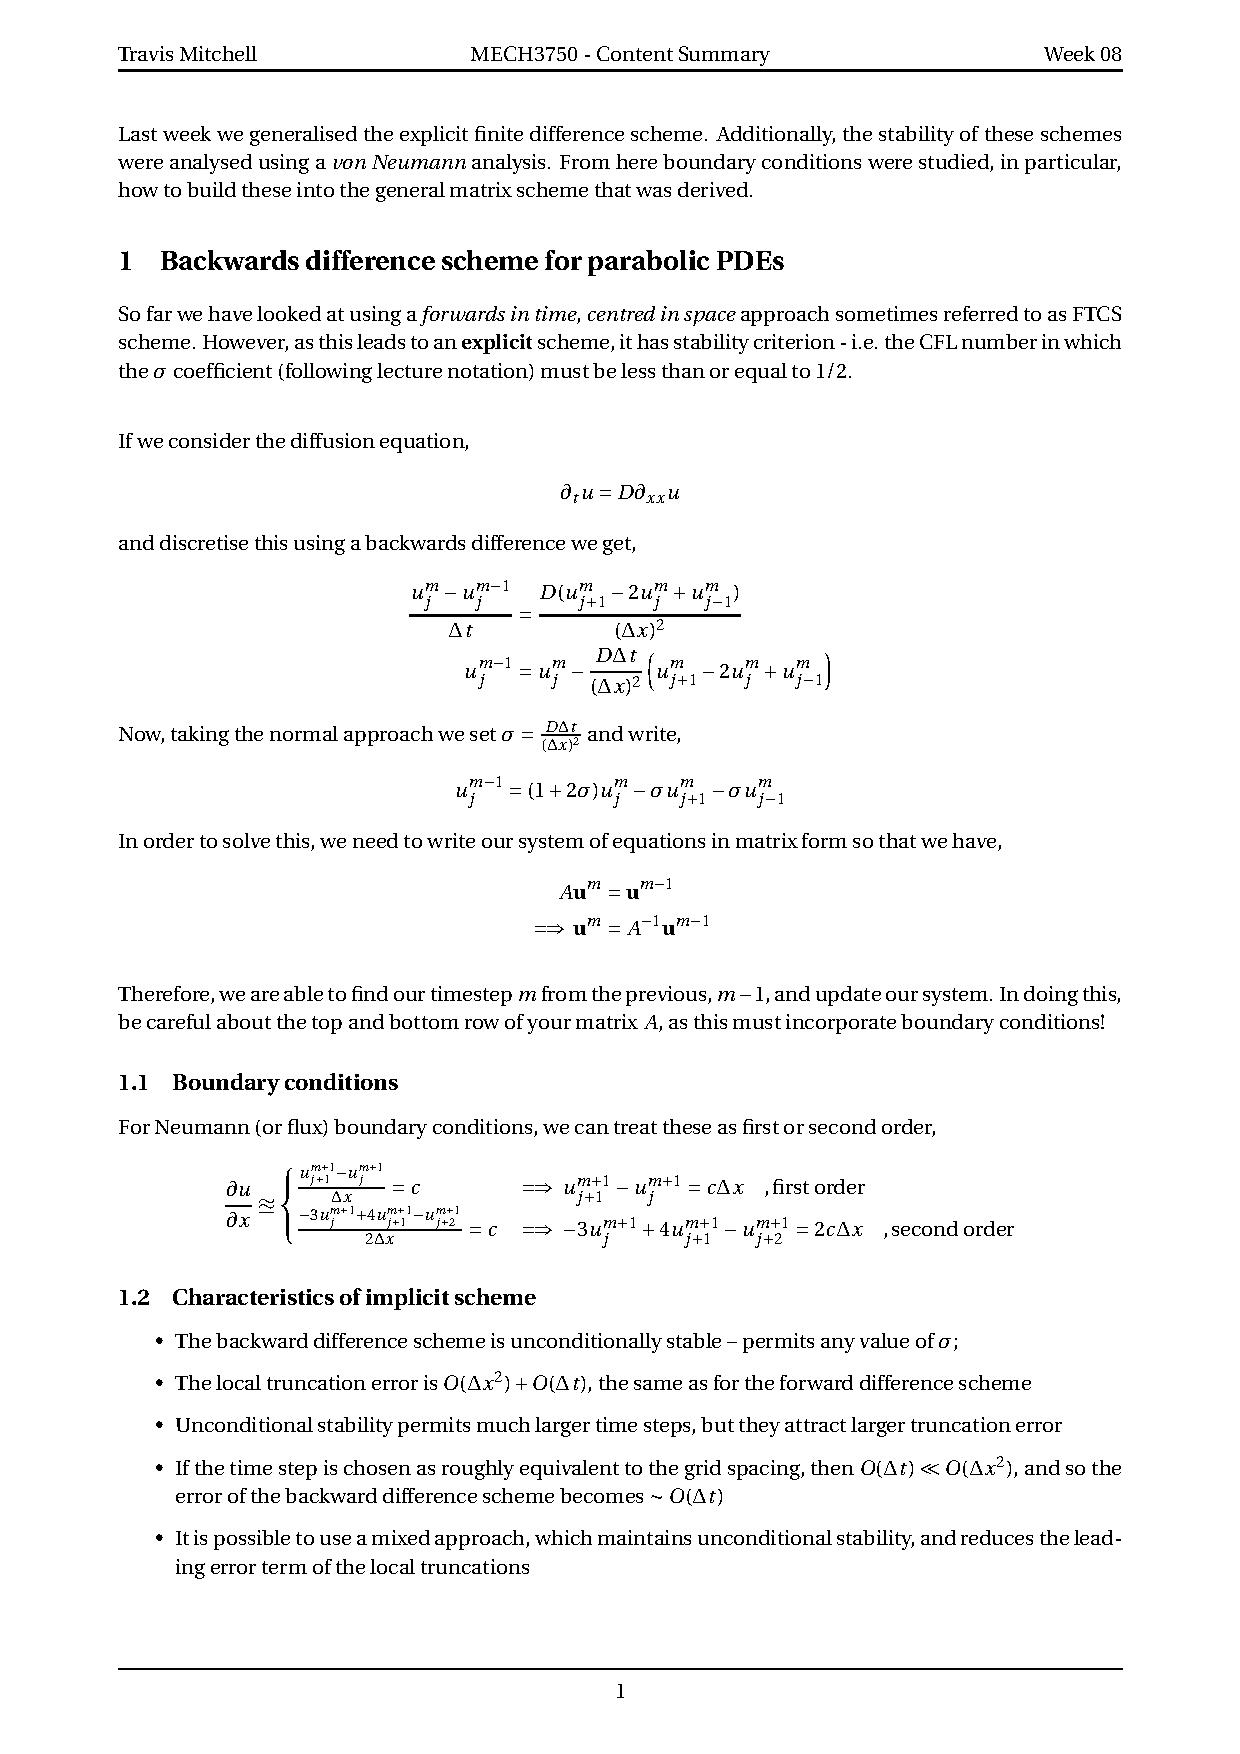
\includepdf[pages={1-}]{wk08/Week08.pdf}
	
	
	\begingroup
	\makeatletter
	\let\clearpage\relax
	\vspace*{\fill}%
	\vspace*{\dimexpr-50\p@-\baselineskip}
	\chapter*{Week 09}
	\textbf{Tutors:} Luke Bartholomew, Nathan di Vaira, Bryce Hill, Kyle Mclaren, Travis Mitchell, Alex Muirhead, William Snell \\\\
	\textbf{Assessment:} 
	\begin{itemize}
		\item Quiz is in Week 9;
		\item Next assignment due in Week 12. 
	\end{itemize}	
	\textbf{Content:}
	\begin{itemize}
		\item Hyperbolic PDEs - what are they and where are they used;
		\item Hyperbolic PDEs - how can we solve them?
	\end{itemize}
	\vspace*{\fill}
	\endgroup
	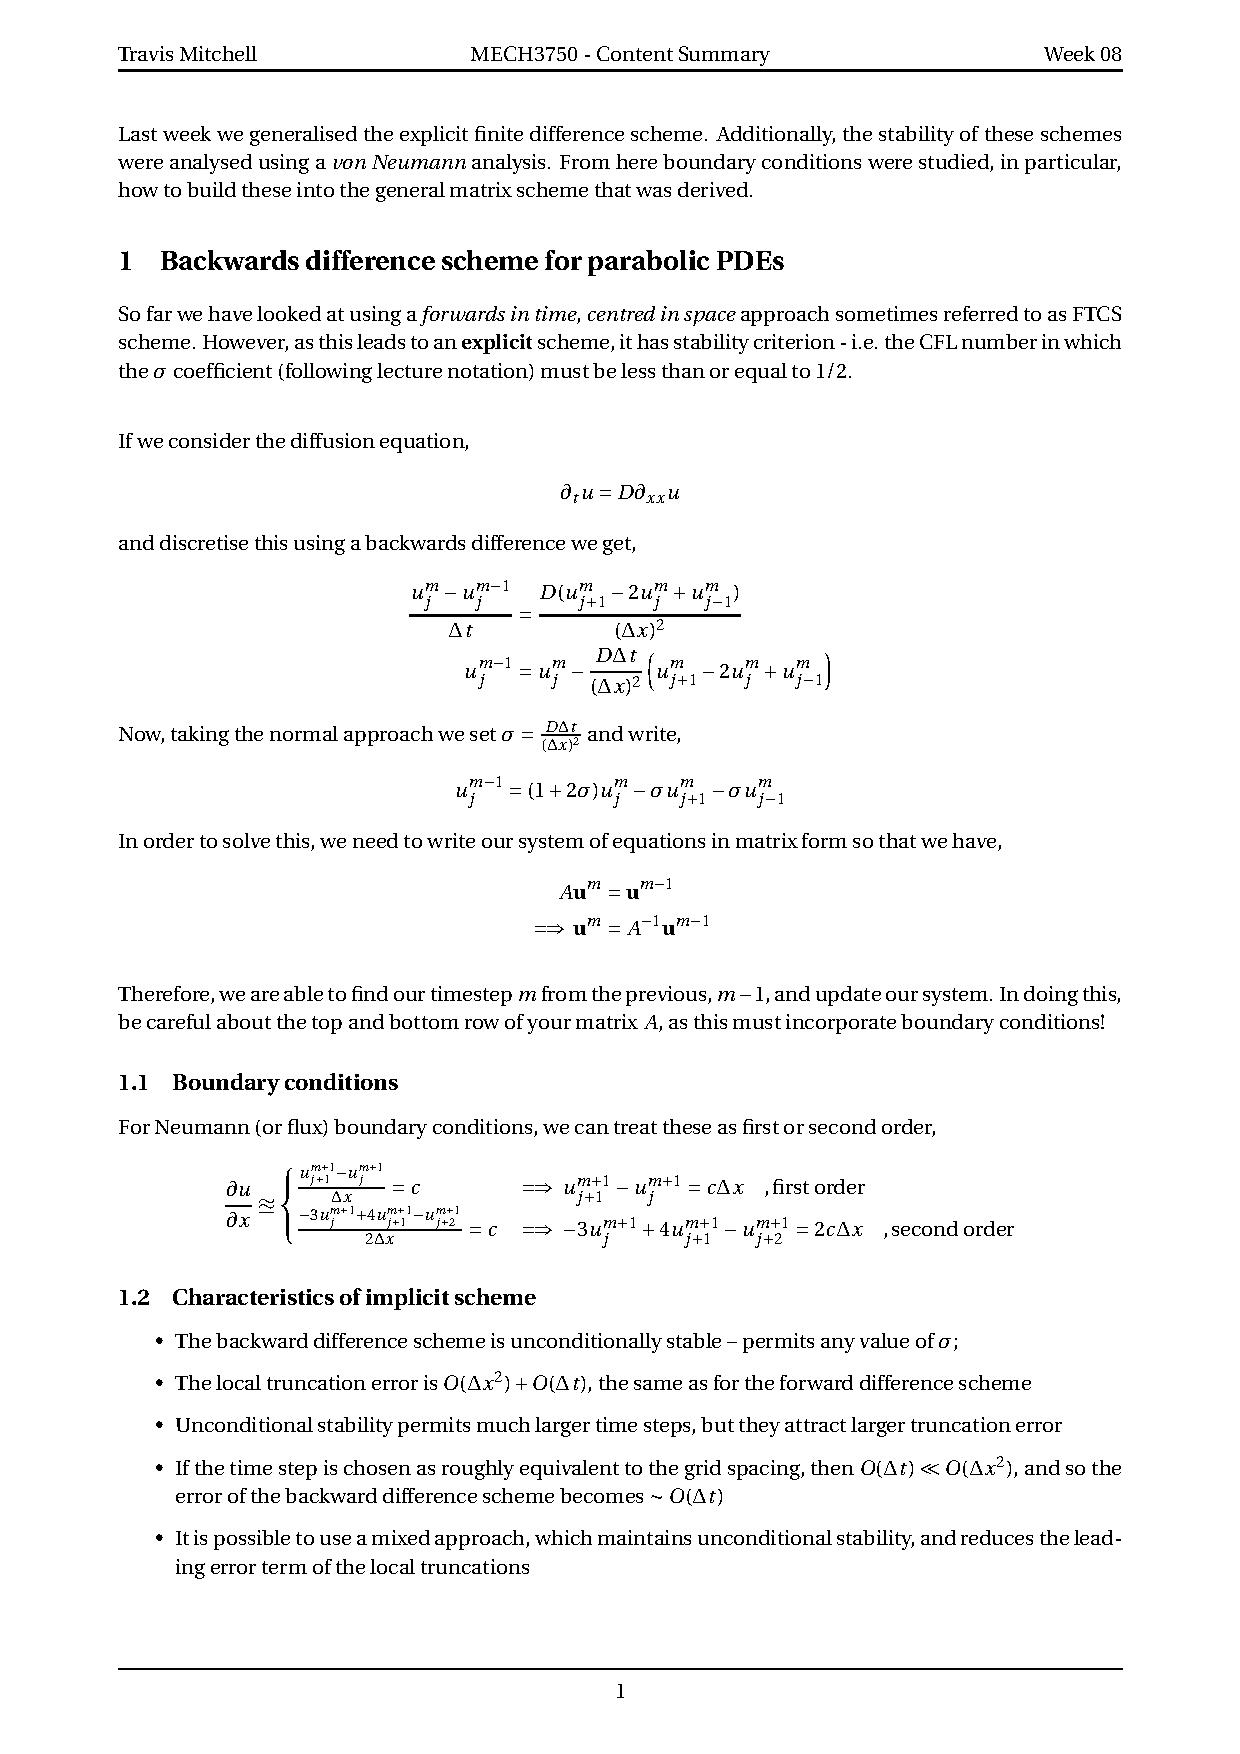
\includepdf[pages={1-}]{wk08/Week08.pdf}
\end{document}
